%%%%%%%%%%%%%%%%%%%%%%%%%%%%%%%%%%%%%%%%%%%%%%%%%%%%%%%%%%%%%%%%%%%
%                                                                 %
%                            CHAPTER FOUR                         %
%                                                                 %
%%%%%%%%%%%%%%%%%%%%%%%%%%%%%%%%%%%%%%%%%%%%%%%%%%%%%%%%%%%%%%%%%%%

\chapter{VERSIONING TABULAR DATA}\label{ch:spreadsheet}

This chapter uses the Copper and Noble Gas databases to demonstrate the implementation of the model presented in the previous chapter.

\section{Validate Comparisons}

The first step is to establish that the two objects being compared meet the requirements of being each other's versions.
For the Copper dataset, the objects result from a compilation effort from the same sources of data.
An entry recording the source material for each row in the table accompanies each reading.
As a result, these entries were used to determine that they share similar provenance.
They will also both be used as data inputs at the same step to generate data visualizations.
The datasets become interchangeable within the context of executing the workflow.
Determining whether the Noble Gas files are versions is a more challenging activity.
From provenance graphs like the one constructed for the entry CAM001 in Figure \ref{CAM001ProvGraph}, the entries share a common source document.
Likewise, a significant portion of the other entries also share sources from the same body of work.
The ones that do not are new or removed entries.
As there was no personal involvement in the use of this data set, determining whether they can occupy the same workflow step requires actually looking into the files.
\begin{figure}
	\centering
	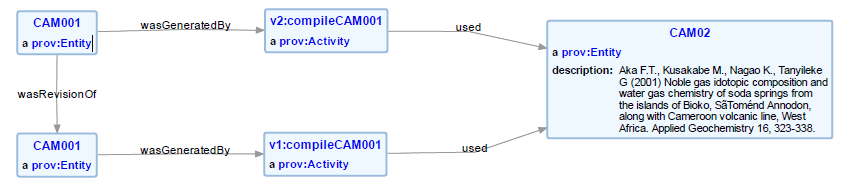
\includegraphics[scale=0.70]{figures/CAM001v1v2.png}
	\caption{Provenance graph for the CAM001 entry of the Noble Gas Database.  Other than the labels, the structure of each data object is very much the same.}
	\label{CAM001ProvGraph}
\end{figure}
Investigating column headers and the accompanying documentation reveals that they report many of the same measurements.
Some amount of leeway is given in this assessment as having every quantity match would mean that the two files aren't versions, but the same object.
This process helps to determine the confidence that using the model to encode the discovered changes will result in a meaningful versioning graph.


\section{Form a Mapping} \label{mapping}

The next step involves formulating a method to determine whether a relationship constitutes an add, invalidate, or modify mapping.
As discussed in the previous chapter, this relies on determining whether an attribute exists in one version, the other, or both.
However, with tabular data, a row and column attribute is required to match specific cells.
For the Noble Gas dataset, this is the entry identifier and the column headers.
Row and column numbers are avoided because edits can result in the same entry associated with different indices.
In addition, the first version of the Noble Gas dataset was organized into multiple files so the same row index would appear more than once, and therefore, could not be used to match related entries.
An observation that also simplifies identifying edits is that cells are rarely added or removed individually.
When one row gains a cell all other rows gain one as well, perhaps with null values, forming a new column.
As a result, data additions and invalidations only use one identifier.
A basic method to determine the identifiers involved in an addition is straight forward.
A set of identifiers \(\mathcal{A} = \mathcal{R}_{r} - \mathcal{R}_{l}\) where \(\mathcal{R}_{l}\) and \(\mathcal{R}_{r}\) correspond to the row identifiers of the left-hand and right-hand versions, respectively.
A converse procedure reveals the set of invalidated attributes \(\mathcal{I} = \mathcal{R}_{l} - \mathcal{R}_{r}\).
All the remaining identifiers exist in both versions and form a set of possible modification attributes.
These are only possibilities because the mapping procedure does not check for differences, and as a result, rows that have not undergone a change are also included.
The same is done with columns.
This only performs a very basic version mapping, but data producers can significantly improve this with their more intimate understanding of the versions.
For example, the base method would not understand that a Location column has been divided into two columns Latitude and Longitude.
A data producer could manually link the Location attribute to the Latitude and Longitude attributes, forming a single modification instead of an invalidate and two additions.

The Copper Minerals dataset starts each row with a unique mineral name, which can be matched across datasets to determine if an entry has undergone a modification.
The column headers have different formats because the initial file is an Excel file and the other is a comma separated file.
As a result, the column headers were manually matched together with the remaining headers in each file mapped into the added and invalidated sets.
The Noble Gas database also uses unique identifiers to mark each of its entries, but the first version of the database divides data among multiple files.
For this reason, the identifiers must first be collected into a single dictionary data structure mapping identifiers to their files.
The version map is then computed from this data structure.
The database also uses multi-line headers which makes a basic automated approach difficult since the cells are not well aligned.
This means that the columns for this database also had to be mapped manually to find the matching columns.

\section{Produce Change Log}

While a linked data versioning graph can now be generated using the mapping method, it is difficult to visualize without using more specialized software.
The solution is to create a human readable change log to both validate the mapping matches and generate human readable change documentation.
This addresses a gap in the Noble Gas data set's documentation which describes data use, but not data changes.
The log is divided into three sections corresponding to the sets generated in Section \ref{mapping}.
However, this provides an opportunity to address a weakness in modern change logs in that they are only human readable.
Two technologies previously introduced, RDFa and JSON-LD, provide a means of embedding linked data into HTML documents, allowing the log to be both human and machine readable.

\begin{figure}
	\centering
	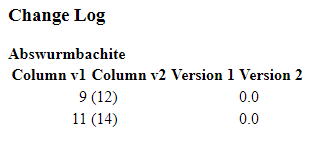
\includegraphics[scale=0.80]{figures/Changelog-zoomed.png}
	\caption{Abswurmbachite entry in the Copper Dataset Change Log}
	\label{changelog_zoomed}
\end{figure}

Consider the entry in Figure \ref{changelog_zoomed} from a change log of the Copper data set.
RDFa uses the attributes in HTML documents to include linked data describing content on the page.
This means that an automated web agent can read the document and extract the associated versioning graph.
A selection of the marked up source from Figure \ref{changelog_zoomed} appears in Listing \ref{rdfa_list}.
Only the lines displaying table headers and the second data line have been removed.
Immediately, it can be seen that the markup is quite cluttered as a result of the clash between RDFa's intent and its use.
The goal of this technology is to describe the content on a page and give context to particular values, marking a string of digits as a phone number for example.
However, in this application, very little of the content is used in the model except for line 3, which uses the mineral name as an attribute label.
It is instead used to encode the versioning model into the HTML document's lattice, leveraging the ability to imply relationships in nested tags.
Unfortunately, RDFa interpreters are very particular in the way they resolve implications, and the order in which data appears in a change log to be human readable does not match the order they need to be for RDFa to encode the model.
In lines 10 and 11, two triples have to be explicitly included in order to conform with the model outlined in Chapter \ref{ch:model}.

\begin{lstlisting}[language=HTML, caption=Abswurmbachite RDFa, label=rdfa_list]
<h3>Change Log</h3>
<div about="Version1" rel="vo:hasAttribute">
  <div resource="v2:Abswurmbachite" typeof="vo:Attribute">
    <span style="font-weight:bold" property="http://www.w3.org/2000/01/rdf-schema#label">Abswurmbachite</span>
    <table rel="vo:Undergoes">
      <tr  about="ChangeAbswurmbachite12" typeof="vo:Change">
        <td align="right" rev="vo:Undergoes" resource="v1:AttributeAbswurmbachite12v1" typeof="vo:Attribute"> 9</td>
        <td property="vo:resultsIn" resource="v2:AttributeAbswurmbachite12v2" typeof="vo:Attribute">(12)</td>
        <td>          </td>
        <td>       0.0</td>
        <span about="Version1" property="vo:hasAttribute" resource="v1:AttributeAbswurmbachite12v1"></span>
        <span about="Version2" property="vo:hasAttribute" resource="v2:AttributeAbswurmbachite12v2"></span>
      </tr>
    </table></div></div><br>
\end{lstlisting}

The difficulties adopting RDFa into the change log arise from a misalignment in intent and use.
Alternatively, a technology meant to store data in web documents, such as JSON-LD, may produce better results.
Listing \ref{json_list} provides the alternative encoding of the Abswurmbachite entry from RDFa.
While significantly longer, the number of triples is not limited by the tag count within a change.
It also separates the human-readable content from the model data, making the source easier to code and modify.
Additionally, a decision was made to divide each change's linked data into its associated row instead of collecting them all at the bottom or top of the page in a single script node.
The practice of a one-node collection is generally helpful for many web applications to load data quickly, but since this is not an application, it makes more sense to break up the content.
Changes to individual attributes can be identified using anchors on the web page, then agents need only extract and parse the link data to these specific entries.
This way, a subgraph of only the pertinent attributes can be created without first ingesting the entire versioning graph.
However, a problem both of these change logs struggle with is size.
The Copper Minerals data set encoded in RDFa is 1.7 MB and JSON-LD is 3.3 MB.
In the Noble Gas data set, the RDFa and JSON-LD change log sizes are 59 and 60 MB, respectively.
The Noble Gas change logs often do not load in a browser.

\begin{lstlisting}[language=HTML, caption=Abswurmbachite JSON-LD, label=json_list]
<h3>Change Log</h3>
<div about="v1:Abswurmbachite">
  <span style="font-weight:bold" property="http://www.w3.org/2000/01/rdf-schema#label">Abswurmbachite</span>
  <table>
    <tr  id="ModifyChangeAbswurmbachite12">
      <td align="right"> 9</td>
      <td >(12)</td>
      <td>          </td>
      <td>       0.0</td>
      <script type="application/ld+json">
[
{
	"@context": "https://orion.tw.rpi.edu/~blee/provdist/GCMD/VO.jsonld", 
	"@id": "http://CUdb.com/v1/AttributeAbswurmbachite9", 
	"@reverse": {
		"hasAttribute": "Version1"
	}, 
	"@type": "vo:Attribute", 
	"label": "Primary", 
	"undergoes": "http://orion.tw.rpi.edu/~blee/provdist/CU/DTDI/CUjsonlog.html#ModifyChangeAbswurmbachite12"
}, 
{
	"@context": "https://orion.tw.rpi.edu/~blee/provdist/GCMD/VO.jsonld", 
	"@id": "http://orion.tw.rpi.edu/~blee/provdist/CU/DTDI/CUjsonlog.html#ModifyChangeAbswurmbachite12", 
	"@type": "vo:ModifyChange", 
	"resultsIn": "http://CUdb.com/v2/AttributeAbswurmbachite12"
}, 
{
	"@context": "https://orion.tw.rpi.edu/~blee/provdist/GCMD/VO.jsonld", 
	"@id": "http://CUdb.com/v2/AttributeAbswurmbachite12", 
	"@reverse": {
		"hasAttribute": "Version2"
	}, 
	"@type": "vo:Attribute", 
	"label": "Primary"
}
]
      </script>
    </tr>
  </table></div><br>
\end{lstlisting}

\section{Generate Versioning Graph}

A versioning graph is now generated using the mapping method determined in Section \ref{mapping}.
Since the attributes in sets \(\mathcal{A}\) and \(\mathcal{I}\) guarantee a change, each item is encoded into linked data and output to a document.

\begin{lstlisting}[language=SPARQL, caption=Noble Gas Add in Turtle, label=NGA]
<http://rdfa.info/play/Version1> a vo:Version ;
	vo:absentFrom <http://rdfa.info/play/AddChange21> .
<http://rdfa.info/play/AddChange21> a <https://orion.tw.rpi.edu/~blee/VersionOntology.owl#AddChange> ;
	vo:resultsIn <http://rdfa.info/play/Attribute21> .
<http://rdfa.info/play/Attribute21> a <https://orion.tw.rpi.edu/~blee/VersionOntology.owl#Attribute> ;
	rdfs:label "EGY001"
<http://rdfa.info/play/Version2> a vo:Version ;
	vo:hasAttribute <http://rdfa.info/play/Attribute21>
\end{lstlisting}
Listing \ref{NGA} presents the statements in turtle format necessary to express that the entry EGY001 has been added to the dataset from Version 1 to Version 2 as shown in Figure \ref{NobleGraph1}.
Notice that the namespace for many of the URIs is \textlangle http://rdfa.info/play/\textrangle.
This results from the triples being extracted out of an HTML change log with embedded linked data, and this is used as the default namespace for the page.
Since we know the number of additions, each change instance can be easily numbered.
Add changes are also kept separate to allow for individual annotation.
Likewise, the graph generator iterates over the set of invalidations and generates a set of statements to instantiate each invalidate change.

\begin{figure}
	\centering
	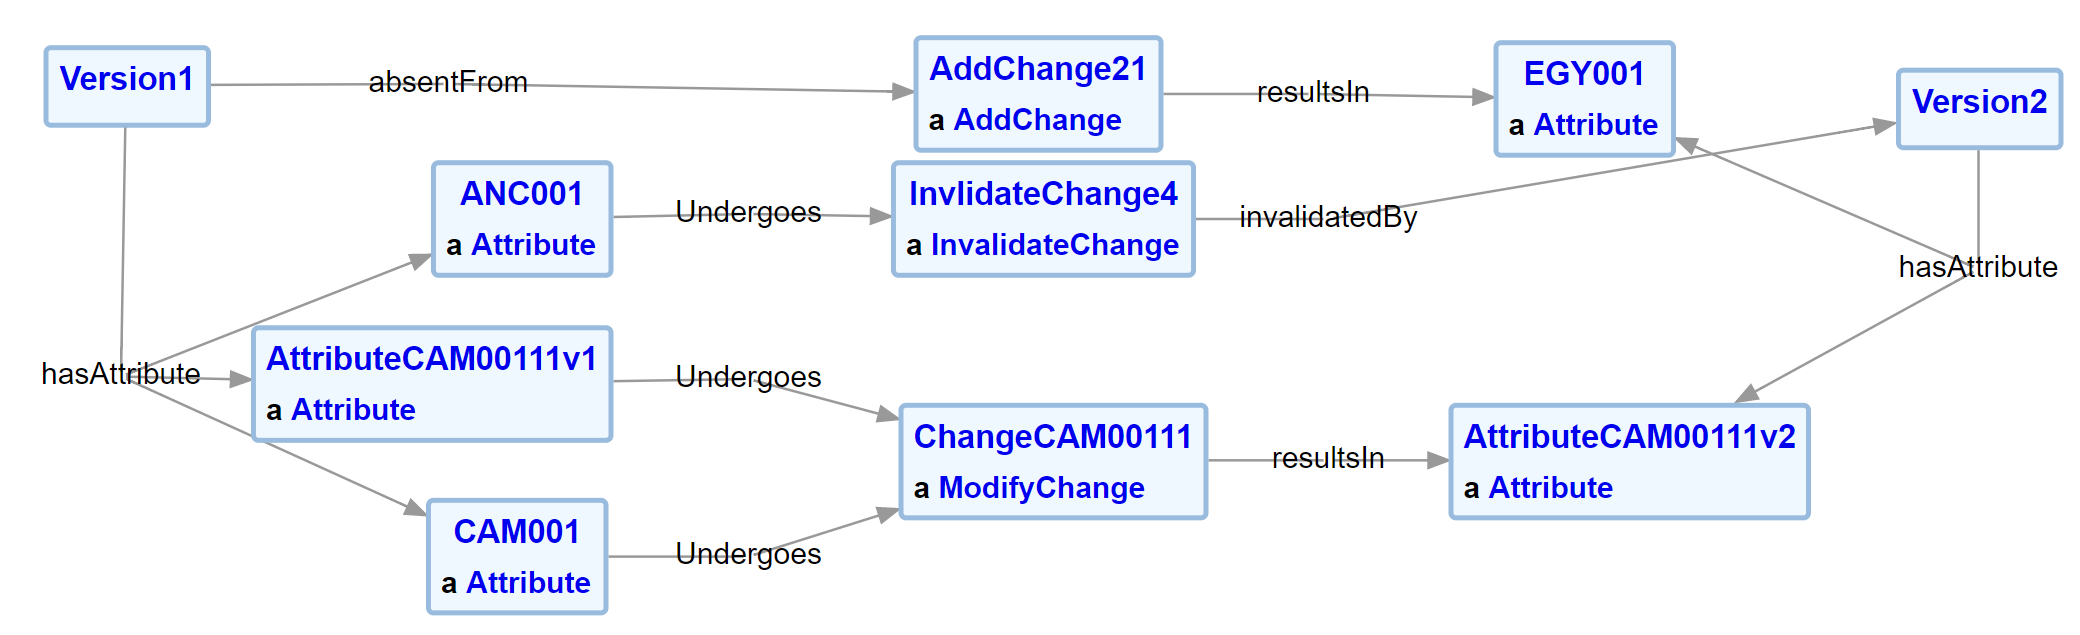
\includegraphics[scale=0.30]{figures/NobleVersion.png}
	\caption{Some initial entries from versions 1 and 2 of the Noble Gas dataset}
	\label{NobleGraph1}
\end{figure}

However, Figure \ref{NobleGraph1} also demonstrates an interesting set of decisions made early in the generation process regarding modifications.
Firstly, the relation presented in the figure is unbalanced and the right-hand side of ChangeCAM00111 links only to the column identifier but not to the corresponding row attribute.
This links from a mismatch between the model's structure, the order in which data appears in the change log, and the way RDFa links properties together.
Because the row label forms the outermost encapsulation, it cannot instantiate both row identifiers and implicitly link them separately.
To do so would require explicitly instantiating the attribute in a non-visible part of the document which would defeat the purpose of using RDFa to implicitly encode the versioning graph into the document.
Secondly, the column identifier AttributeCAM00111v1 combines together the row label and the column number, making it unique to just the CAM001 row.
This was a decision to properly identify the attribute as it appears in the change log document.
Since the item is not a generic column 11 element in the log, but a specific item of CAM001, the entry id is included in the column identifier.
This formulation poses a problem when trying to query the graph and determine how many rows have a column 11 modify change for example.
When the versioning triples are not extracted from a change log and printed as linked data, the structure has greater freedom as seen in Figure \ref{NobleGraph2}.

\begin{figure}
	\centering
	\begin{adjustbox}{addcode={\begin{minipage}{\width}}{
					\caption{Versioning Graph representing the linked data graph with selected entries of additions, invalidations, and modifications. 
			}\end{minipage}},rotate=90,center}
		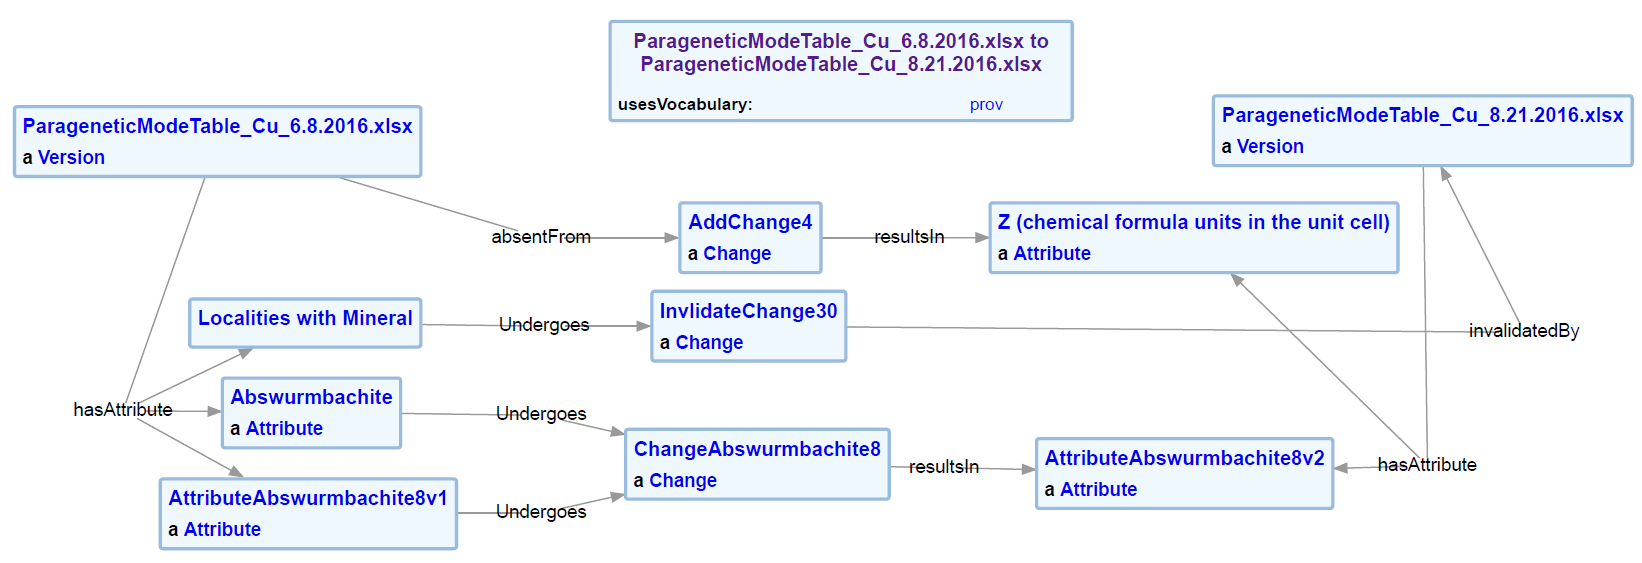
\includegraphics[scale=0.5]{figures/VersioningGraph2.png}%
	\end{adjustbox}
	\label{CopperGraphVerGraph}
\end{figure}

\section{Multiple Linked Versions}

The figures in this document so far have depicted a comparison between only two versions, but versioning often involves more than two objects, either in sequence or parallel.
Figure \ref{NobleGraph2} shows a graph that follows change as it moves through three versions of the Noble Gas data set.
From the first to second version of the data, EGY001 becomes introduced as an attribute into the dataset.
This entry then undergoes a modification change in columns 29, 31, and 43 when comparing versions two and three.
The construction results in a format naturally oriented to show the flow of change from version one to three.
The advantage of this formation is that now many versions can be related together using a unified set of semantics that cannot be achieved through combining the other concepts and properties in Chapter \ref{ch:model}.
Versioning forms a continuous relationship even into later versions without introducing new semantics.
This is important since many versioning linked data alternatives view version change as a single contained activity.

When considering multiple versions, a particular challenge is when an attribute does not change.
In that particular case, no links are created, but if this occurs between two transitions, the flow of change is broken.
For example, in Figure \ref{NobleGraph2}, column 31 of EGY001 becomes modified transitioning into the third version.
If that column underwent no activity in the next transition but changed from version four to five, the connection between all the column 31s would no longer be continuous.
This poses a problem for executing queries in a triple store which rely on graph traversals, but no path exists between the two modification changes in the example.


\begin{figure}
	\centering
	\begin{adjustbox}{addcode={\begin{minipage}{\width}}{
					\caption{Versioning Graph representing the linked data graph with selected entries of additions, invalidations, and modifications after the publication of the third version. 
			}\end{minipage}},rotate=90,center}
		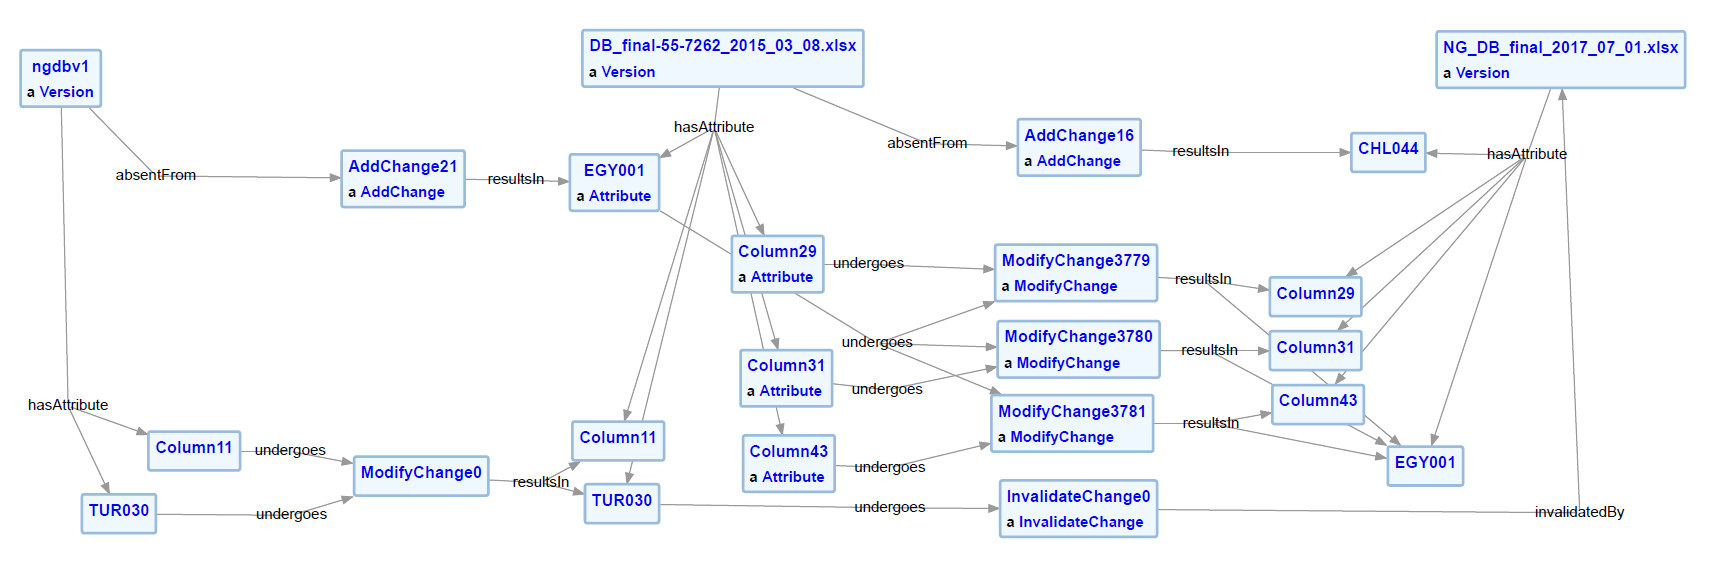
\includegraphics[scale=0.5]{figures/NobleVersion2.png}%
	\end{adjustbox}
	\label{NobleGraph2}
\end{figure}